\section{PCE Maps} 
\subsection{Quantum channels} % {{{
Quantum channels comprehend the most general linear operations that a quantum
system undergo independently of its past~\cite{zimansbook,cirac}. To introduce
their construction and properties, first let us define several objects. We will
denote Hilbert spaces as \hilbert and $d$-dimensional Hilbert spaces as
$\hilbert_d$. The set of linear operators over a Hilbert space \hilbert will
be written as $\mcB(\hilbert)$.
%, the subset of density matrices as
%$\mcS(\hilbert)$, which is in turn a subset of the so called trace-class
%operators $\mcT(\hilbert)$, for the finite dimensional case, the one studied
%here, $\mcT(\hilbert)$ and $\mcB(\hilbert)$ coincide~\cite{zimansbook}. 

The construction of quantum channels includes basically three ingredients:
linearity, trace preserving and complete positivity. The trace preserving
property is needed to
send convex combinations of density matrices into the convex combination of the
evolution of such density matrices, this is, let $\mcE$ such linear operation,
thus $p \rho_1 +(1-p) \rho_2 \mapsto p \mcE[\rho_1]+(1-p)\mcE[\rho_2]$. The
trace preserving property is required for the process $\mcE$ to be deterministic, \ie{} $\tr\mcE[\rho]=\tr \rho =1$ is the probability that the process $\mcE$ will
happen to the state $\rho\in \mcS(\hilbert)$. The complete
positivity condition is needed to preserve positive semidefiniteness and handle
the non-local feature of quantum theory. A map $\mcE$ is positive if $\mcE[\Delta]\geq 0 \ \ \forall \Delta \in \mcB(\hilbert), \ \ \Delta\geq 0$\cpnote{Francois, de tu nota, la $\Delta$ ya es hermitica, pues 
decimos que es una matriz de densidad} \ddnote{$\Delta$ no es hermítico, sin embargo la definición de positividad-semidefinida se extiende a la parte hermítica por convención, revisé y en ningún libro mencionan la hermiticidad en este punto. Sin embargo esos casos no son relevantes en este contexto por supuesto}. In the other hand, a map is completely positive if
 $\id_k \otimes \mcE$ is a positive map for $k=1,2,\dots$, where 
between the system and an ancilla with Hilbert space $\hilbert_k$. This ensures that every positive semidefinite operator of any
extension of the system (where the quantum channel is now a local operation) is
mapped into positive semidefinite operators. The trace preserving is automatically
fulfilled for all extensions if $\mcE$ fulfills it. Therefore, any density matrix of a system
where $\mcE$ acts locally, is sent to a valid density matrix, this is the
substance of complete positivity.
\flnote{No creo que lo de Bell state sea conveniente. Mejor decir algo como: 
E is totally positive if trivially extending E to the tensor product of H with an arbitrary dimensional ancilla space yields a positive operation. }\ddnote{ejecutado}

Quantum channels can be characterized by means of the Choi-\jami{}
isomorphism~\cite{choi,jamil}. This is, given a linear operation
$\mcE:\mcB(\hilbert)\to \mcB(\hilbert)$, the so-called Choi matrix of it is
$\choi=\left(\id \otimes \mcE\right)[\proj{\Omega}{\Omega}]$ (also called dynamical matrix), where
$\ket{\Omega}=1/\dim(\hilbert)\sum_i^{\dim(\hilbert)}\ket{i}\ket{i}$ is the
Bell state between two copies of \hilbert. The map \mcE is completely positive if and only
\choi is positive-semidefinite.

Furthermore, quantum channels enjoy the well-known \textit{Kraus representation} (or
operator-sum representation) which reads 
\begin{equation}
\mcE[\rho]=\sum_i K_i \rho
K_i^\dagger{}
\end{equation}
with $\sum_i K_i^\dagger{}K_i=\one$ (the trace preserving condition). In fact, a linear operation is completely positive if and only
if it has a Kraus representation~\cite{Kraus1983}. The minimum number of Kraus operators $K_i$ needed to represent the channel is called \textit{Kraus rank}. 
%
It can be seen from Kraus decomposition that quantum channels preserve
hermiticity, this has a practical consequence when using hermitian bases, \ie{} let $\left\{ \Delta_i \right\}$ a hermitian basis in $\mcB(\hilbert)$, then the entries of the matrix representation of the quantum channel $\mcE$, $\hat
\mcE_{ij}=\tr\left( \Delta_i \mcE[\Delta_j] \right)$, are real. In particular in this work we use bases consisting in the so-called \textit{Pauli strings}, defined as 
\begin{equation}
\sigma_{\vec \alpha}:=\sigma_{\alpha_1}\otimes \sigma_{\alpha_2} \otimes \dots \otimes \sigma_{\alpha_N},
\label{eq:pauli_strings}
\end{equation}
where $N$ is the number of two-level particles (\aka{} qubits), $\alpha_i=0,1,2,3$ and $\sigma_0:=\one$, $\sigma_{1,2,3}:=\sigma_{x,y,z}$. Thus, the bases $\left\{ 2^{N/2} \sigma_{\vec \alpha} \right\}$ are orthonormal in $\mcB(\hilbert)$. Also notice that $\tr \sigma_{\vec \alpha}=\delta_{\vec\alpha,\vec 0} 2^{N}$.

\flnote{
probablemente convenga mostrar la ecuaci'on desplegada. Asimismo se debe decir que 
$\sum_i K_i^\dagger K_i = 1$ para la trace-preserving property. 
Creo qie ``hermiticity preserving'' es en parte consecuencia de la definición, pero esto no es muy importante
}\ddnote{ejecutado, hacia falta edicion, sin embargo lo de hermiticity preserving es para hacer incapie en por que podemos trabajar en una representacion totalmente real de los canales.}

  \ddnote{[Choi representation, Kraus operators and Stinespring dilation]}

% }}}
\subsection{Single qubit case} % {{{
\label{sec:single:qubit}
\todo{David escribe una primera version y luego Carlos itera}
\pce{} maps are defined as those valid quantum channels that \textit{nullify} \textit{Pauli strings} \ddnote{aqui introduzco el nombre estandar}, in the case of one qubit, they consist of maps nullifying the averages $r_\alpha:=\langle \sigma_\alpha \rangle$ with $\alpha=1,2,3$. The three components $r_\alpha$ form the well-known \textit{Bloch vector} $\vec r$, describing one qubit density matrices,
\begin{equation}
\rho=\frac{\one +\vec r \cdot \vec \sigma}{2}.
\end{equation}
Therefore, maps erasing components of $\vec r$ are parametrized in the following way,
\begin{equation}
r_\alpha \mapsto \tau_\alpha r_\alpha
\end{equation}
where $\tau_k$ is either $1$ or $0$. It is well-known that not every operation like this is a quantum map, for example collapsing the entire Bloch ball into a disk of radio equal to one is not a quantum channel. A direct evaluation of the complete positivity conditions~\cite{zimansbook,davalosdivisibility},
\begin{align}
1+\tau_1+\tau_2+\tau_3 &\geq 0 \nonumber \\
1+\tau_i-\tau_j-\tau_k &\geq 0 \ \ \forall i\neq j \neq k,
\end{align}
show that only five operations are \pce: the identity map, the completely depolarizing channel ($\rho \mapsto \one/2$); and bit, phase, and bit-phase flip channels~\cite{chuangbook}. These channels can be pictured with one column tables, see~\fref{fig:one:qubit:examples}. Finally notice that the condition $\tau_0=1$ is needed to have trace-preserving maps.
These operations have been studied in \cite{Ziman2005,davalosdivisibility} and are by definition diagonal in the Pauli basis $1/\sqrt{2} \left\{ \one, \sigma_x,\sigma_y,\sigma_z \right\}$, \ie{} $\hat \mcE=\diag{\left(1,\tau_x, \tau_y, \tau_z \right)}$. They form a tetrahedron in the space of eigenvalues 
 
with
\begin{equation}
\mcL_\alpha[\Delta]:= \frac{\gamma}{2}\left( \sigma_\alpha \Delta \sigma_\alpha -\Delta \right).
\label{eq:1qubit_semigroup}
\end{equation}
We will show later that this can be trivially generalized to the $N$ qubit case.



\begin{align}
U_\alpha\ket{\psi} \ket{0}:=\frac{1}{\sqrt{2}} \left( \ket{\psi} \ket{0}+\sigma_\alpha \ket{\psi}\ket{1} \right)\\
U_\alpha\ket{\psi} \ket{1}:=\frac{1}{\sqrt{2}} \left( \ket{\psi} \ket{0}-\sigma_\alpha \ket{\psi}\ket{1} \right)
\label{eq:1qubit_stinespring}
\end{align}
similar to the semigroup generator, we will show later that this can be trivially generalized to the $N$ qubit case.


\begin{itemize}
\item The single qubit case, describe some of the features.
\item Single qubit Kraus operators.
\item Single qubit relation with decoherence. 
\end{itemize}
% }}}
\subsection{Pauli component erasing maps} % {{{

The density matrix $\rho$ of a system of $N$ qubits can be written in Pauli
matrices basis as 
\begin{equation}\label{eq:N_qubits_rho}
	\rho =\frac{1}{2^N} 
            \sum_\valpha r_\valpha \sigma_\valpha,
%             \quad r_{\vec0}=1,
% 	\sigma_{\alpha_1}\otimes \ldots \otimes \sigma_{\alpha_N},
%             \sum_{\alpha_1,\ldots,\alpha_N=0}^3 \paulicomponents
% 	\sigma_{\alpha_1}\otimes \ldots \otimes \sigma_{\alpha_N},
	%r_{0,\ldots,0}=1,
\end{equation}
where $\vec \alpha$ denotes a vector index $\qty(\alpha_1,\ldots,\alpha_N)$,
$\sigma_{\vec \alpha} := \sigma_{\alpha_1}\otimes \ldots \otimes
\sigma_{\alpha_N}$ is the tensor product of Pauli matrices, and 
$r_{\vec \alpha}$ is the coefficient corresponding to the expansion
of the density matrix in the complete orthonormal basis $\left\{ 2^{-N/2}\sigma_{\vec
\alpha} \right\}$. In the sum each of the $N$ components of $\valpha$, i.e.
$\alpha_{1,\cdots,N}$ is varied from $0$ to $3$. 
Notice that $\sigma_{\vec 0} = \openone$, and since both $\tr \rho=1$ and 
$\tr \sigma_\valpha=2^N\delta_{\valpha,\vec 0}$, then $r_{\vec 0}=1$. 
We shall refer to $\paulicomponents$ as the ``Pauli components'' of the density
matrix of a system of qubits. 

Consider the linear operations that simply attenuate the Pauli components of 
a multiqubit system:
\begin{equation}
	\paulicomponents \mapsto \taus \paulicomponents.
% 	\taus = 0,1, \hspace{1.5cm}	\tau_{0,\ldots,0}=1.
\label{eq:definition:Pauli}
\end{equation}
For the operation to preserve the trace of the density matrix, we require that
$\tau_{\vec 0}=1$.  
% These operations are diagonal in the basis $\left\{
% 2^{-N/2}\sigma_{\vec \alpha} \right\}$, which follows from
% \eref{eq:sigma_property}. 
% The diagonal components are $\taus$, i.e. $\hat
% \mcE=\diag(\taus)$. Additionally, they belong to the subset of unital channels
% that can be written as convex combinations of unitary channels. \cpnote{Alguien 
% puso aca que lo probarian, pero no lo hemos discutido y quizá no le veo 
% el caso en este articulo}
\cpnote{Creo qeu vale la pena mencionar la relacion con los canales de Ruskai. 
Lo discutimos en pleno, o por lo menos cuando esten JA y FL. quizá tambien discutir
si se mencionan a los canales  \cite{Siudzinska2020}}

\cpnote{davalos, dale aca un pequeño rollo relevante quiza de una o dos
frases de la importancia de esta familia.} \ddnote{De momento no he encontrado
alguna reference, para qubits si, pero para los generales no}.



A Pauli component erasing (PCE) operation is a Pauli diagonal operation
%  A linear operation 
% $\mcE$ 
that either preserves or completely erases the Pauli components of a
density matrix. That is, 
% it transforms its Pauli components as 
\begin{equation} \label{eq:PCE_definition}
% \begin{split}
% 	\paulicomponents \mapsto \ \taus \paulicomponents,\hspace{.5cm}\\
% 	\taus = 0,1, \hspace{1.5cm}	\tau_{0,\ldots,0}=1.
	\paulicomponents \mapsto \taus \paulicomponents,\quad 
	\taus = 0,1.
% \end{split}
\end{equation}
It is worth noticing that not all PCE maps are quantum operations. For single 
qubits, if just one of the $\taus=0$, the complete positivity condition 
is not met, as discussed in \sref{sec:single:qubit}. It will be of central interest
in this article to determine which $\taus$ lead to a valid quantum map.

%\ddnote{hay un typo en esta ecuacion}
% A PCE operation is a trace-preserving operation that leaves invariant or erases 
% the Pauli components of a density matrix of $n$ qubits. \janote{Ojo que aquí 
% habrá que unificar la notación de subíndices. No lo hago porque no lo tengo del 
% todo claro y no hay problema en dejarlo así por el momento.}
% \cpnote{Aca voy} 

A graphical representation for PCE maps may be introduced, being the
two qubits case what has proved to be the most useful. Consider a $N$ dimensional 
Cartesian grid, with $4^N$ places.  Each place has $N$ integer coordinates, ranging
from 0 to 3, so each place corresponds to a given $\vec \alpha$ in 
\eref{eq:N_qubits_rho}. For a given PCE, we shall fill 
the square if the corresponding $\tau_{\vec \alpha}=1$. Otherwise, we leave it 
empty. Examples for $N=1$ are provided in \fref{fig:one:qubit:examples}, whereas
for two qubits, we exemplify them in \fref{fig:two:qubit:examples}. 
% Notice
% than in both cases we drop the label $\alpha$ for simplicity, as it will 
% remain unchanged throughout this text \janote{No entiendo qué estás diciendo
% aquí}. 

\begin{figure} % {{{
\begin{center}
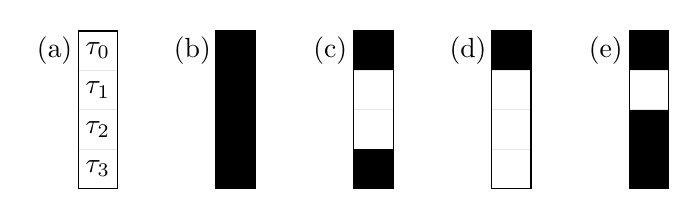
\begin{tikzpicture}[x=0.5cm, y=0.5cm] % {{{
\pgfmathsetmacro{\unitstep}{3.5}
% Coordenadas   {{{
\node at (-0.6,0.5) {(a)} ;
\draw[black!10] (0,0) rectangle (1,1); \node at (0.5,0.5) {$\tau_0$} ;
\begin{scope}[shift={(0,-1)}]
\draw[black!10] (0,0) rectangle (1,1); \node at (0.5,0.5) {$\tau_1$} ;
\end{scope}
\begin{scope}[shift={(0,-2)}]
\draw[black!10] (0,0) rectangle (1,1); \node at (0.5,0.5) {$\tau_2$} ;
\end{scope}
\begin{scope}[shift={(0,-3)}]
\draw[black!10] (0,0) rectangle (1,1); \node at (0.5,0.5) {$\tau_3$} ;
\end{scope} 
\draw (0,-3) rectangle (1,1); 
% }}}
\begin{scope}[shift={(1*\unitstep,0)}] % Identity {{{
% \begin{scope}[shift={(\unitstep*2,0)}]
\node at (-0.6,0.5) {(b)} ;
\fill[black] (0,0) rectangle (1,1);
\draw[black!10] (0,0) rectangle (1,1);
\begin{scope}[shift={(0,-1)}] \draw[black!10] (0,0) rectangle (1,1); \end{scope}
\begin{scope}[shift={(0,-2)}] \draw[black!10] (0,0) rectangle (1,1); \end{scope}
\begin{scope}[shift={(0,-3)}] \draw[black!10] (0,0) rectangle (1,1); \end{scope}
\draw (0,-3) rectangle (1,1); 
\begin{scope}[shift={(0,-1)}] \fill[black] (0,0) rectangle (1,1); \end{scope}
\begin{scope}[shift={(0,-2)}] \fill[black] (0,0) rectangle (1,1); \end{scope}
\begin{scope}[shift={(0,-3)}] \fill[black] (0,0) rectangle (1,1); \end{scope}
\end{scope} % }}}
\begin{scope}[shift={(2*\unitstep,0)}] % Dephasing {{{
\node at (-0.6,0.5) {(c)} ;
\fill[black] (0,0) rectangle (1,1);
% \draw (0,0) rectangle (1,1);
\draw[black!10] (0,0) rectangle (1,1);
\begin{scope}[shift={(0,-1)}] \draw[black!10] (0,0) rectangle (1,1); \end{scope}
\begin{scope}[shift={(0,-2)}] \draw[black!10] (0,0) rectangle (1,1); \end{scope}
\begin{scope}[shift={(0,-3)}] \draw[black!10] (0,0) rectangle (1,1); \end{scope}
\draw (0,-3) rectangle (1,1); 
% \begin{scope}[shift={(0,-1)}] \fill[black] (0,0) rectangle (1,1); \end{scope}
% \begin{scope}[shift={(0,-1)}] \draw (0,0) rectangle (1,1); \end{scope}
% \begin{scope}[shift={(0,-2)}] \fill[black] (0,0) rectangle (1,1); \end{scope}
% \begin{scope}[shift={(0,-2)}] \draw (0,0) rectangle (1,1); \end{scope}
\begin{scope}[shift={(0,-3)}] \fill[black] (0,0) rectangle (1,1); \end{scope}
% \begin{scope}[shift={(0,-3)}] \draw (0,0) rectangle (1,1); \end{scope}
\end{scope} % }}}
\begin{scope}[shift={(3*\unitstep,0)}] % Depolarization {{{
\node at (-0.6,0.5) {(d)} ;
\fill[black] (0,0) rectangle (1,1);
% \draw (0,0) rectangle (1,1);
\draw[black!10] (0,0) rectangle (1,1);
\begin{scope}[shift={(0,-1)}] \draw[black!10] (0,0) rectangle (1,1); \end{scope}
\begin{scope}[shift={(0,-2)}] \draw[black!10] (0,0) rectangle (1,1); \end{scope}
\begin{scope}[shift={(0,-3)}] \draw[black!10] (0,0) rectangle (1,1); \end{scope}
\draw (0,-3) rectangle (1,1); 
% \begin{scope}[shift={(0,-1)}] \fill[black] (0,0) rectangle (1,1); \end{scope}
% \begin{scope}[shift={(0,-1)}] \draw (0,0) rectangle (1,1); \end{scope}
% \begin{scope}[shift={(0,-2)}] \fill[black] (0,0) rectangle (1,1); \end{scope}
% \begin{scope}[shift={(0,-2)}] \draw (0,0) rectangle (1,1); \end{scope}
% \begin{scope}[shift={(0,-3)}] \fill[black] (0,0) rectangle (1,1); \end{scope}
% \begin{scope}[shift={(0,-3)}] \draw (0,0) rectangle (1,1); \end{scope}
\end{scope} % }}}
\begin{scope}[shift={(4*\unitstep,0)}] % (e) canal malo {{{
\node at (-0.6,0.5) {(e)} ;
\fill[black] (0,0) rectangle (1,1);
% \draw (0,0) rectangle (1,1);
\draw[black!10] (0,0) rectangle (1,1);
\begin{scope}[shift={(0,-1)}] \draw[black!10] (0,0) rectangle (1,1); \end{scope}
\begin{scope}[shift={(0,-2)}] \draw[black!10] (0,0) rectangle (1,1); \end{scope}
\begin{scope}[shift={(0,-3)}] \draw[black!10] (0,0) rectangle (1,1); \end{scope}
% \begin{scope}[shift={(0,-1)}] \fill[black] (0,0) rectangle (1,1); \end{scope}
% \begin{scope}[shift={(0,-1)}] \draw (0,0) rectangle (1,1); \end{scope}
\begin{scope}[shift={(0,-2)}] \fill[black] (0,0) rectangle (1,1); \end{scope}
% \begin{scope}[shift={(0,-2)}] \draw (0,0) rectangle (1,1); \end{scope}
\begin{scope}[shift={(0,-3)}] \fill[black] (0,0) rectangle (1,1); \end{scope}
% \begin{scope}[shift={(0,-3)}] \draw (0,0) rectangle (1,1); \end{scope}
\draw (0,-3) rectangle (1,1); 
\end{scope} % }}}
\end{tikzpicture} % }}}
\end{center}
	\caption{In (a) we introduce the positions of the single 
qubit diagrams, so that each square corresponds to a single 
$\tau_{\alpha}$, $\alpha=0,1,2,3$. The diagrams in 
(b), (c) and (d) correspond to the identity map, dephasing channel, and 
total depolarization, respectively. In (e) we show a map that only erases the component
$r_1$ and thus does not correspond to a quantum operation.}
	\label{fig:one:qubit:examples}
\end{figure} % }}}

\begin{figure} % {{{
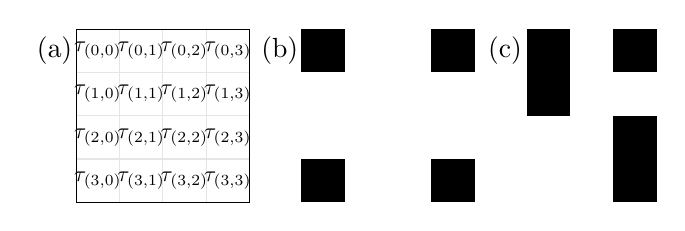
\begin{tikzpicture}[x=0.55cm, y=0.55cm] % {{{
\pgfmathsetmacro{\unitstep}{5.2}
\begin{scope}[shift={(0*\unitstep,0)}] % Coordenadas {{{
\node at (-0.5,0.5) {(a)} ;
% \cuadritotikz{}
    \foreach \x in {0,1,2,3} {
      \foreach \y in {0,1,2,3} {
        \begin{scope}[shift={(\x,-\y)}] 
          \draw[black!10] (0,0) rectangle (1,1); 
%           \draw (0,0) rectangle (1,1); 
          \node at (0.5,0.5) {\scalebox{.8}{$\tau_{(\y,\x)}$}};
         \end{scope}
%         \node at (0,-\y) (input\y) {$i_\y$};
%         \node[block] at (2,-\y) (block\y) {$f_\y$};
%         \draw[->] (input\y) -- (block\y);
%         \draw[->] (block\y.east) -- +(0.5,0);
    }
    }
 \draw (0,-3) rectangle (4,1);
\end{scope} % }}}
\begin{scope}[shift={(1*\unitstep,0)}] % Good channel {{{
\node at (-0.5,0.5) {(b)} ;
\cuadritotikz{}
%     \foreach \x in {0,1,2,3} {
%       \foreach \y in {0,1,2,3} {
%         \begin{scope}[shift={(\x,-\y)}] 
%           \draw (0,0) rectangle (1,1); 
% %           \node at (0.5,0.5) {$\tau_{\y,\x}$};
%          \end{scope}
% %         \node at (0,-\y) (input\y) {$i_\y$};
% %         \node[block] at (2,-\y) (block\y) {$f_\y$};
% %         \draw[->] (input\y) -- (block\y);
% %         \draw[->] (block\y.east) -- +(0.5,0);
%     }
%     }
\begin{scope}[shift={(0,-3)}] \fill[black] (0,0) rectangle (1,1); \end{scope}
\begin{scope}[shift={(3,-3)}] \fill[black] (0,0) rectangle (1,1); \end{scope}
\begin{scope}[shift={(0,0)}] \fill[black] (0,0) rectangle (1,1); \end{scope}
\begin{scope}[shift={(3,0)}] \fill[black] (0,0) rectangle (1,1); \end{scope}
\end{scope} % }}}
\begin{scope}[shift={(2*\unitstep,0)}] % Good channel {{{
\node at (-0.5,0.5) {(c)} ;
\cuadritotikz{}
%     \foreach \x in {0,1,2,3} {
%       \foreach \y in {0,1,2,3} {
%         \begin{scope}[shift={(\x,-\y)}] 
%           \draw (0,0) rectangle (1,1); 
% %           \node at (0.5,0.5) {$\tau_{\y,\x}$};
%          \end{scope}
% %         \node at (0,-\y) (input\y) {$i_\y$};
% %         \node[block] at (2,-\y) (block\y) {$f_\y$};
% %         \draw[->] (input\y) -- (block\y);
% %         \draw[->] (block\y.east) -- +(0.5,0);
%     }
%     }
\begin{scope}[shift={(0,0)}] \fill[black] (0,0) rectangle (1,1); \end{scope}
\begin{scope}[shift={(0,-1)}] \fill[black] (0,0) rectangle (1,1); \end{scope}
\begin{scope}[shift={(2,0)}] \fill[black] (0,0) rectangle (1,1); \end{scope}
\begin{scope}[shift={(2,-2)}] \fill[black] (0,0) rectangle (1,1); \end{scope}
\begin{scope}[shift={(2,-3)}] \fill[black] (0,0) rectangle (1,1); \end{scope}
\end{scope} % }}}
\end{tikzpicture} % }}}
	\caption{In (a) we introduce the
positions of two qubit diagrams. The diagrams in 
(b) corresponds to a quantum channel that results from the tensor product of
bit flip channels in each qubit [see \fref{fig:one:qubit:examples}(c)],
and in (c) a diagram of a map that is not a quantum channel is presented.}
	\label{fig:two:qubit:examples}
\end{figure} % }}}

% In \Fref{fig:PCE_figs} we introduce a pictorial representation of PCE operations of 
% 1, 2 and 3 qubits. Every position in the column, board or cube is associated with 
% the subindices of $\taus$ of a PCE operation. If a little square or cube  in position
% $\alpha_1,\ldots,\alpha_N$ is black, then $\taus=1$, if it is white, then $\taus=0$. For example,
% \begin{center}
% 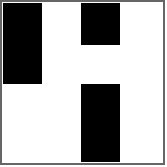
\includegraphics[width=2cm]{2qubits_pce_example}
% \end{center}
% this represents a PCE operation of 2 qubits that leaves invariant the Pauli 
% components $r_{0,0}$, $r_{0,2}$, $r_{1,0}$, $r_{2,2}$, $r_{3,2}$. This operation
% is not completely positive and therefore is not a quantum channel. In contrast, 
% \begin{center}
% \includegraphics[width=2cm]{2qubits_pceChannel_example01}
% \end{center}
% this other example of PCE operation that leaves invariant Pauli components 
% $r_{0,0}$, $r_{1,2}$, $r_{2,1}$, $r_{3,3}$ satisfies complete positivity and 
% is a quantum channel. 
% 
% 



% }}}




